\chapter{Results and analysis}
\emph{The goal of this chapter is to find answers to the project subtasks. Top performing algorithms for predicting TIRS road surface temperature, precipitation amount and DST111 road surface temperature are identified, as well as the top performing algorithm for classifying precipitation type.}

\section{Experimental setup and summary of results}
	A solution to each of the project subtasks are covered in the following sections. The results are achieved methodically for each subtask (see experimental methodology \ref{sec:method_results}). A summary of the methodology of finding an optimized algorithm for predicting/classifying target feature $f_t$:
	\begin{enumerate}
		\item Rank the possible input features $f_i$ in terms of linear correlation to $f_t$ to get a ranking of the input features. The ranking is referred to as top input features.
		\item Run $n$ spot-checking experiments on the algorithms that can classify/predict $f_t$, where $n$ is the amount of input features available in total. The idea is to find which input features give the best performance- and generalization score for each algorithm. The $i$th spot-checking run uses the top $i$ input features, where $1 \leq i \leq n$. An accumulated score $P_{acc}$ is calculated which takes both performance and overfitting into account.
		\item Optimize the hyperparameters of Lasso, MLP and kNN using their optimized choice of top input features.
		\item Analyze the best scores for each algorithm using their optimized choice of top input features and hyperparameter settings. The algorithm whose accumulated performance score is best, is identified as the top performing algorithm.
	\end{enumerate}

	Table \ref{table:results_summary} shows a summary of the top performing algorithms that were found for modelling each target feature related to the project subtasks.
	
	\begin{table}[H]
		\centering
		\caption{Shows the top performing algorithms for each of the project subtasks. }
		\resizebox{\textwidth}{!}{%
		\begin{tabular}[7]{l | l | l | l | l | c | c  }
    			Sensor & Subtask & Problem type & Best algorithm & Choice of top performing input features & Optimized settings & Best performance \\ \hline %(0.84, 0.46, -0.41)
			Optic eye & model precipitation type & classification problem & CART & \makecell{road surface condition \\ road friction \\ DST111 road surface temperature \\ hour \\ month } & Scikit default & $(Accuracy, \overline{F1}_{test}) = (0.84, 0.46)$ \\ \hline
			Optic eye & model precipitation amount & regression problem & kNN & \makecell{road friction} &  $K=64$ &  $MSE_{test}=0.31$ \\ \hline
			TIRS & model TIRS road surface temperature & regression problem & MLP & \makecell{DST111 road surface temperature \\ road surface condition \\ road friction \\ month \\ hour \\ precipitation type} &  n.o. hidden nodes: 64 &  $MSE_{test}=0.88$ \\ \hline
 			DST111 & model DST111 road surface temperature & regression problem & Random forest &  \makecell{road surface condition \\ road friction \\ month \\ precipitation type \\ hour} &  Scikit default &  $MSE_{test} = 10.16$ 
			\label{table:results_summary}
		\end{tabular}
		}
	\end{table}

	The sections that follow describe how the results in table \ref{table:results_summary} were obtained.

\section{Predicting road surface temperature (TIRS)} 
	\subsection{Input features correlation ranking}
	\begin{table}[H]
		\centering
		\caption{Relevancy of each possible input feature to the target feature: TIRS road surface temperature. }
		\begin{tabular}[3]{c | l | l }
    			Relevancy ranking & Input feature & Correlation score  \\
			 \hline
			1 & DST111 road surface temperature & 7688772.49 \\ \hline
			2 & road surface condition & 11048.87 \\ \hline
			3 & road friction & 6840.20 \\ \hline
			4 & month & 4300.00 \\ \hline
			5 & hour & 1968.02 \\ \hline
			6 & precipitation type & 1784.49 \\ \hline
			7 & precipitation amount & 238.91 
 
			\label{table:feature_comparison_tirs}
		\end{tabular}
	\end{table}

	The correlation ranking in table \ref{table:feature_comparison_tirs} shows that DST111 is the most relevant feature while Optic Eye features are less relevant in predicting TIRS road surface temperature.

	\subsection{Spot-checking}
	\begin{table}[H]
		\centering
		\caption{Results from spot-checking experiment on the top features for predicting TIRS road surface temperature. The results are shown as a tuple: ($MSE_{test}$, $MSE_{diff}$) where $MSE_{test}$ represents performance and $MSE_{diff} = MSE_{test} - MSE_{train}$ shows the degree of overfitting, larger values of $MSE_{diff}$ indicate overfitting.}
		\resizebox{\textwidth}{!}{%
		\begin{tabular}[8]{l |c | c | c | c |c | c |c }
    			Algorithm & MSE top 7 & MSE top 6 & MSE top 5 & MSE top 4 & MSE top 3 & MSE top 2 & MSE top 1 \\
			 \hline 
			OLS 			& (1.19, 0.02) & (1.19, 0.02) & (1.19, 0.02)  & (1.20, 0.02)  & (1.22, 0.02) & (1.22, 0.02) & (1.22, 0.02) \\ \hline
			CART 		&  (1.36, 1.10) & (1.35, 1.08) & (1.31, 1.03) & (1.05, 0.30) & (1.03, 0.15) & (1.02, 0.09) & (1.01, 0.05) \\ \hline
			kNN 			& (0.94, 0.32) & (0.93, 0.32) & (0.92, 0.31) & (1.08, 0.18) & (1.16, 0.09) & (1.16, 0.06) & (1.21, 0.04) \\ \hline
			MLP & (0.90, 0.01) & (0.86, 0.02) & (0.86, 0.01) & (0.97, 0.03) & (1.00, 0.02) & (1.02, 0.02) & (1.01, 0.01)\\ \hline
			Lasso 		& (1.24, 0.02) & (1.24, 0.02) & (1.24, 0.02) & (1.24, 0.02) & (1.24, 0.02) & (1.24, 0.02) & (1.24, 0.02) \\ \hline
			Random forest 	&  (1.01, 0.65) & (1.00, 0.66) & (1.01, 0.64) & (1.01, 0.23) & (1.01, 0.12) & (1.01, 0.08) & (1.01, 0.05)
 
			\label{table:spotcheck_tirs}
		\end{tabular}
		}
	\end{table}
	
	\begin{table}[H]
		\centering
		\caption{Shows an accumalated performance score $P_{acc} = MSE_{test} + MSE_{diff}$. Top results for each algorithm are highlighted. In case of ties, the one using the fewest number of input features is considered optimized.}
		\resizebox{\textwidth}{!}{%
		\begin{tabular}[8]{l |c | c | c | c |c | c |c }
    			Algorithm & $P_{acc}$ top 7 features & $P_{acc}$ top 6 features & $P_{acc}$ top 5 features & $P_{acc}$ top 4 features & $P_{acc}$ top 3 features & $P_{acc}$ top 2 features & $P_{acc}$ top 1 features\\
			\hline
			OLS 			& 1.21 &  1.21 & \textbf{\underline{1.21}} & 1.22 & 1.24 & 1.24 & 1,24 \\ \hline
			CART 		&  2.46 & 2.43 & 2.34 & 1.35 & 1.18 & 1.11 & \textbf{\underline{1.06}} \\ \hline
			kNN 			& 1.26 & 1.25 & 1.25 & 1.26 & 1.25 & \textbf{\underline{1.22}} & 1.25 \\ \hline
			MLP &  0.91 & 0.88 & \textbf{\underline{0.87}} & 1.00 & 1.02 & 1.04 & 1.02 \\ \hline
			Lasso 		& 1.26 & 1.26 & 1.26 & 1.26 & 1.26 & 1.26 & \textbf{\underline{1.26}} \\ \hline
			Random forest 	&  1.66 & 1.66 & 1.65 & 1.24 & 1.13 & 1.09 & \textbf{\underline{1.06}}
 
			\label{table:spotcheck_tirs_acc}
		\end{tabular}
		}
	\end{table}

	The results from table \ref{table:spotcheck_tirs_acc} show that OLS and MLP have best accumulated scores when using the top five features, whereas kNN is optimized when the top two features are used. CART, Lasso and Random forest have optimized scores in using the top one feature.

	\subsection{Optimizing hyperparameters}
	\begin{table}[H]
		\centering
		\caption{Shows the effect of optimizing the hyperparameters of kNN, MLP and Lasso using their top input features}
		\resizebox{\textwidth}{!}{%
		\begin{tabular}[6]{l |c | c | c | c | c }
    			Algorithm & Default hyperparameter setting & Optimized setting & Default performance $P_{acc}$ & optimized performance ($MSE_{test}$, $MSE_{diff}$) & optimized performance $P_{acc}$ \\
			\hline
			kNN 			& $k = 5$ & $k = 64$ & 1.22 & (1.00, 0.04) & 1.04 \\ \hline
 			MLP & n.o. hidden nodes: 100 & n.o. hidden nodes: 64 & 0.87 & (0.88, 0.01) & 0.89\\ \hline
			Lasso		& $\lambda = 1$ & $\lambda = 0.001$ & 1.26 & (1.22, 0.02) & 1.24
			\label{table:optimization_tirs}
		\end{tabular}
		}
	\end{table}

	As shown in table \ref{table:optimization_tirs}, accumulated scores were improved for kNN and Lasso when optimized hyperparameter settings were used. MLP showed a slightly reduced accumulated score using optimized hyperparameters. However, since the default settings were used as well in the optimization process, it is believed that setting number of hidden nodes to 64 is indeed an optimized choice and thus an optimized overall performance was obtained.

	\subsection{Results and analysis} \label{sec:results_tirs}

	\begin{table}[H]
		\centering
		\caption{Shows the overall optimized settings and performances for each of the algorithms in predicting TIRS road surface temperature. The top performing algorithm is highlighted.}
		\resizebox{\textwidth}{!}{%
		\begin{tabular}[5]{l |c | c | c | c }
    			Algorithm & Optimized settings & Best choice of input features & Best performance ($MSE_{test}$, $MSE_{diff}$) & Best performance $P_{acc}$ \\
			\hline
			OLS 				& Scikit default & top 5 & (1.19, 0.02) & 1.21 \\ \hline
			CART 			& Scikit default & top 1 & (1.01, 0.05) & 1.06\\ \hline
 			kNN 				& $k= 64$ & top 2 & (1.00, 0.04) & 1.04 \\ \hline
			\textbf{\underline{MLP}}		& \textbf{\underline{n.o. hidden nodes: 64}} & \textbf{\underline{top 5}} & \textbf{\underline{(0.88, 0.01)}} & \textbf{\underline{0.89}} \\ \hline
			Lasso			& $\lambda = 0.001$ & top 1 & (1.22, 0.02) & 1.24\\ \hline
			Random forest		& Scikit default & top 1 & (1.01, 0.05) & 1.06
			\label{table:best_performances_tirs}
		\end{tabular}
		}
	\end{table}

	Table \ref{table:best_performances_tirs} shows that MLP has the lowest $P_{acc}$ score among all algorithms and is thus the algorithm that performs best in terms of performance- and generalization when it comes to predicting TIRS road surface temperature. MLP have a performance score of $MSE_{test} = 0.88$ which means that in predicting TIRS road surface temperature, MLP was on average off by $\sqrt{0.88} \approx 0.94 \celsius$ from the actual temperature measurements in the test dataset. Figure \ref{fig:scatter_mlp} shows the relationship between predictions made by MLP on the test dataset and actual values. %lägg in plot som visar predictions

\begin{figure}[H] 
	\centering
	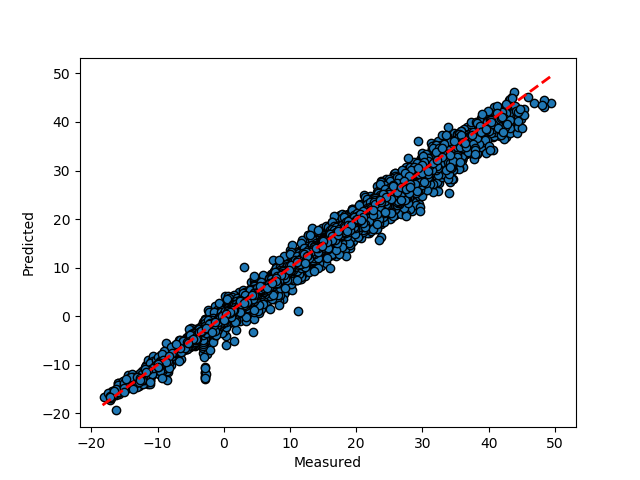
\includegraphics[width=0.8\textwidth]{media/tirs_predictions.png}
	\caption{Shows the relationship between actual measurements and predictions made by MLP to predict TIRS road surface temperature. The closer a point is to the red dashed line, the more accurate prediction for that observation. }
	\label{fig:scatter_mlp}
\end{figure}
	
\section{Classifying precipitation type (Optic Eye)}
\subsection{Input features correlation ranking}
	\begin{table}[H]
		\centering
		\caption{Relevancy of each possible input feature to the target feature: precipitation type }
		\begin{tabular}[3]{c | l | l }
    			Relevancy ranking & Input feature & Correlation score  \\
			 \hline
			1 & road surface condition & 4506.14 \\ \hline
			2 & road friction & 4274.88 \\ \hline
			3 & DST111 road surface temperature & 1263.89 \\ \hline
			4 & Hour & 609.45 \\ \hline
			5 & Month & 16.71 
 
			\label{table:feature_comparison_prectype}
		\end{tabular}
	\end{table}

	The correlation ranking in table \ref{table:feature_comparison_prectype} shows that the road surface condition and road friction are most relevant when it comes to classifying precipitation type whereas the time-related input features are less relevant.

	\subsection{Spot-checking}
	\begin{table}[H]
		\centering
		\caption{Results from spot-checking experiment on the top features in classifying precipitation type. The results are shown as a triple: (accuracy, $\overline{F1}_{test}$, $\overline{F1}_{diff}$) where $\overline{F1}_{test}$ represents performance and $\overline{F1}_{diff} = \overline{F1}_{test} - \overline{F1}_{train}$ shows the degree of overfitting, larger values of $\overline{F1}_{diff}$ indicate overfitting.}
		\resizebox{\textwidth}{!}{%
		\begin{tabular}[6]{l |c | c | c | c |c }
    			Algorithm & Performance top 5 & Performance top 4 & Performance top 3 & Performance top 2 & Performance top 1 \\
			 \hline 
			Logistic regression 	& (0.81, 0.21, 0.00) & (0.81, 0.21, 0.00) & (0.81, 0.21, 0.00)  & (0.82, 0.21, 0.00)  & (0.81, 0.21, 0.00)  \\ \hline
			kNN 				& (0.85, 0.40, -0.05) & (0.85, 0.37, -0.05) & (0.86, 0.39, -0.03) & (0.86, 0.34, 0.00) & (0.83, 0.34, 0.00)  \\ \hline
			CART 			& (0.84, 0.46, -0.41) & (0.85, 0.44, -0.28) & (0.86, 0.41, -0.06) & (0.86, 0.34, 0.00) & (0.83, 0.34, 0.00) \\ \hline
			Naïve bayes		& (0.82, 0.27, 0.00) & (0.82, 0.26, 0.00) & (0.82, 0.26, 0.00) & (0.82, 0.25, 0.00) & (0.82, 0.25, 0.00)  \\ \hline
			MLP 	& (0.85, 0.35, 0.00) & (0.85, 0.38, 0.00) & (0.86, 0.37, 0.00) & (0.86, 0.34, 0.00) & (0.82, 0.21, 0.00) \\ \hline
			Random forest 		& (0.85, 0.45, -0.40) & (0.85, 0.42, -0.29) & (0.86, 0.42, -0.05) & (0.86, 0.34, 0.00) & (0.83, 0.34, 0.00) 
 
			\label{table:spotcheck_prectype}
		\end{tabular}
		}
	\end{table}
	
	\begin{table}[H]
		\centering
		\caption{Shows an accumalated performance score $P_{acc} = \overline{F1}_{test} - \overline{F1}_{diff}$. Top results for each algorithm are highlighted. In case of ties, the one using the fewest number of input features is considered optimized.}
		\resizebox{\textwidth}{!}{%
		\begin{tabular}[6]{l |c | c | c | c |c  }
    			Algorithm & $P_{acc}$ top 5 features& $P_{acc}$ top 4 features & $P_{acc}$ top 3 features & $P_{acc}$ top 2 features & $P_{acc}$ top 1 features \\
			 \hline 
			Logistic regression 	& 0.21 & 0.21 & 0.21 & 0.21 & \textbf{\underline{0.21}} \\ \hline
			kNN 				& \textbf{\underline{0.45}} & 0.42 & 0.42 & 0.34 & 0.34 \\ \hline
			CART 			& \textbf{\underline{0.87}} & 0.72 & 0.47 & 0.34 & 0.34\\ \hline
			Naïve bayes		& \textbf{\underline{0.27}} & 0.26 & 0.26 & 0.25 & 0.25  \\ \hline
			MLP 	& 0.35 & \textbf{\underline{0.38}} & 0.37 & 0.34 & 0.21 \\ \hline
			Random forest 		& \textbf{\underline{0.85}} & 0.71 & 0.47 & 0.34 & 0.34 

			\label{table:spotcheck_prectype_acc}
		\end{tabular}
		}
	\end{table}

	The results from table \ref{table:spotcheck_prectype_acc} show that kNN, CART, Naïve bayes and Random forest perform best when using the top five features, whereas MLP and Logistic regression have optimized performances when using the top four and top one features respectively.

	\subsection{Optimizing hyperparameters}

	\begin{table}[H]
		\centering
		\caption{Shows the effect of optimizing the hyperparameters of kNN and MLP using their top input features}
		\resizebox{\textwidth}{!}{%
		\begin{tabular}[6]{l |c | c | c | c | c }
    			Algorithm & Default hyperparameter setting & Optimized settings & Default performance $P_{acc}$ & optimized performance (accuracy, $\overline{F1}_{test}$, $\overline{F1}_{diff}$) & optimized performance $P_{acc}$ \\ \hline
			kNN 			& \textbf{$k = 5$} & $k = 1$ & 0.45 & (0.81, 0.40, -0.47) & 0.87 \\ \hline
 			MLP & n.o. hidden nodes: 100 & n.o. hidden nodes: 100 & 0.35 & (0.85, 0.33, -0.01) & 0.34
			\label{table:optimization_prectype}
		\end{tabular}
		}
	\end{table}

	As shown in table \ref{table:optimization_prectype}, the optimized settings for MLP is the same as its default settings. Its overall performance was slightly reduced in comparison to the results in table \ref{table:spotcheck_prectype} and \ref{table:spotcheck_prectype_acc}. This is believed to be due to non-deterministic behavior of MLP. Table \ref{table:optimization_prectype} shows that kNN was significantly improved using $k=1$. Based on its new accumulated performance score: $P_{acc} = 0.87$, it tied with CART as the top performing algorithm as seen in table \ref{table:spotcheck_prectype_acc}.

	\subsection{Results and analysis} \label{sec:results_prectype}

	\begin{table}[H]
		\centering
		\caption{Shows the overall optimized settings and performances for each of the algorithms in classifiying precipitation type. The best performing algorithms are highlighted.}
		\resizebox{\textwidth}{!}{%
		\begin{tabular}[5]{l |c | c | c | c }
    			Algorithm & Optimized settings & Best choice of input features & Best performance (Accuracy, $\overline{F1}_{test}$, $\overline{F1}_{diff}$) & Best performance $P_{acc}$ \\
			\hline
			Logistic regression 	& Scikit default & top 1 & (0.81, 0.21, 0.00) & 0.21 \\ \hline
			\textbf{\underline{kNN}} 				& \underline{$\mathbf{k= 1}$} & \textbf{\underline{top 5}} & \textbf{\underline{(0.81, 0.40, -0.47)}} & \textbf{\underline{0.87}} \\ \hline
 			\textbf{\underline{CART}} 			& \textbf{\underline{Scikit default}} & \textbf{\underline{top 5}} & \textbf{\underline{(0.84, 0.46, -0.41)}} & \textbf{\underline{0.87}} \\ \hline
			Naïve bayes		& Scikit default & top 5 & (0.82, 0.27, 0.00) & 0.27 \\ \hline
			MLP		& Scikit default & top 4 & (0.85, 0.38, 0.00) & 0.38 \\ \hline
			Random forest		& Scikit default & top 5 & (0.85, 0.45, -0.40) & 0.85
			\label{table:best_performances_prectype}
		\end{tabular}
		}
	\end{table}

	Table \ref{table:best_performances_prectype} shows that kNN and CART are tied for highest $P_{acc}$ score among all algorithms. To break the tie, CART is chosen over kNN since CART has a higher accuracy- and $\overline{F1}$ score. CART is thus the algorithm that performs best in terms of performance and generalization when it comes to classifying precipitation type. CART has a performance score of $\overline{F1}_{test} = 0.46$ and accuracy $= 0.82$. This means that out of all observations in the test dataset, CART correctly classified 82\% of the precipitation types correctly in the test dataset. 

	However, $\overline{F1}_{test} = 0.46$ indicates that the accuracy score is misleading. The recall scores in table \ref{table:classreport_prectype} reveal that CART performed well in classifying no precipitation: 90\%, and that lower scores were obtained with classifying the other precipitation types. The lowest recall score is classifying rain and snow mixed. Rain and snow mixed was correctly identified in 3\% of the cases when rain and snow mixed appeared in the test dataset. 

	\begin{table}[H]
		\centering
		\caption{Shows how CART performs in classifying each of the different precipitation types using the optimized setup as shown in table \ref{table:best_performances_prectype}}
		\begin{tabular}[6]{c |l | c | c | c | l }
    			Value & Precipitation type & Precision & Recall & F1 & N.o. occurrences \\
			\hline
			1 & no precipitation & 0.90 & 0.92 & 0.91 & 18912 \\ \hline
			2 & rain with $>= 0 \celsius$ air temperature & 0.55 & 0.47 & 0.51 & 3222 \\ \hline
			3 & rain with $< 0 \celsius$ air temperature & 0.26 & 0.28 & 0.27 & 50 \\ \hline
			4 & snow & 0.61 & 0.55 & 0.58 & 781 \\ \hline
			6 & rain and snow mixed & 0.03 & 0.03 & 0.03 & 71
			\label{table:classreport_prectype}
		\end{tabular}
	\end{table}

 %lägg in plot som visar predictions


\section{Predicting precipitation amount (Optic Eye)} 
	\subsection{Input features correlation ranking}

	\begin{table}[H]
		\centering
		\caption{Input features correlation ranking to the target feature: precipitation amount. }
		\begin{tabular}[3]{c | l | l }
    			Relevancy ranking & Input feature & Correlation score  \\
			 \hline
			1 & road friction & 4478.75 \\ \hline
			2 & road surface condition & 2793.48 \\ \hline
			3 & DST111 road surface temperature & 234.64 \\ \hline
			4 & month & 60.36 \\ \hline
			5 & hour & 19.93 
			\label{table:feature_comparison_precamount}
		\end{tabular}
	\end{table}

		Table \ref{table:feature_comparison_precamount} shows that the road friction and road surface condition have high correlation to precipitation amount while the time-related features are less relevant. 

	\subsection{Spot-checking}

	\begin{table}[H]
		\centering
		\caption{Results from spot-checking experiment on the top features for predicting precipitation amount. The results are shown as a tuple: ($MSE_{test}$, $MSE_{diff}$) where $MSE_{test}$ represents performance and $MSE_{diff} = MSE_{test} - MSE_{train}$ shows the degree of overfitting, larger values of $MSE_{diff}$ indicate overfitting.}
		\resizebox{\textwidth}{!}{%
		\begin{tabular}[6]{l |c | c | c | c |c }
    			Algorithm & top 5 features & top 4 features & top 3 features & top 2 features & top 1 features \\
			 \hline 
			OLS 			& (0.58, -0.06) & (0.58, -0.06) & (0.58, -0.06)& (0.58, -0.06) & (0.58, -0.06)\\ \hline
			CART 		& (1.01, 0.94) & (0.63, 0.18) & (0.98, 0.91) & (0.98, 0.80) & (0.62, 0.17)\\ \hline
			kNN 			& (0.60, 0.15) & (0.61, 0.07) & (0.58, 0.15) & (0.62, 0.15) & (0.63, 0.05)\\ \hline
			MLP & (0.56, -0.06) & (0.57, -0.05) & (0.55, -0.05) & (0.56, -0.06) & (0.55, -0.06)\\ \hline
			Lasso 		& (0.61, -0.05) & (0.61, -0.05) & (0.61, -0.05) & (0.61, -0.05) & (0.61, -0.05) \\ \hline
			Random forest 	& (0.67, 0.52) & (0.59, 0.13) & (0.68, 0.51) & (0.71, 0.46) & (0.57, 0.11)
 
			\label{table:spotcheck_precamount_mse}
		\end{tabular}
		}
	\end{table}

	\begin{table}[H]
		\centering
		\caption{Shows an accumalated performance score $P_{acc} = MSE_{test} + MSE_{diff}$. Top results for each algorithm are highlighted. In case of ties, the one with fewest input features is considered optimized.}
		\resizebox{\textwidth}{!}{%
		\begin{tabular}[6]{l |c | c | c | c |c }
    			Algorithm & $P_{acc}$ top 5 features & $P_{acc}$ top 4 features & $P_{acc}$ top 3 features & $P_{acc}$ top 2 features & $P_{acc}$ top 1 features \\
			\hline
			OLS 			& 0.52 & 0.52 & 0.52 & 0.52 & \textbf{\underline{0.52}} \\ \hline
			CART 		& 1.95 & 0.81 & 1.89 & 1.78 & \textbf{\underline{0.79}} \\ \hline
			kNN 			& 0.75 & 0.68 & 0.73 & 0.77 & \textbf{\underline{0.68}} \\ \hline
			MLP & 0.50 & 0.52 & 0.50 & 0.50 & \textbf{\underline{0.49}} \\ \hline
			Lasso 		& 0.56 & 0.56 & 0.56 & 0.56 & \textbf{\underline{0.56}} \\ \hline
			Random forest 	& 1.19 & 0.72 & 1.19 & 1.17 & \textbf{\underline{0.68}} 
 
			\label{table:spotcheck_precamount_acc}
		\end{tabular}
		}
	\end{table}

		The results from table \ref{table:spotcheck_precamount_acc} indicate that all algorithms performs at best when the top one feature is used alone.

	\subsection{Optimizing hyperparameters}

	\begin{table}[H]
		\centering
		\caption{Shows the effect of optimizing the hyperparameters of kNN, MLP and Lasso using their top input features}
		\resizebox{\textwidth}{!}{%
		\begin{tabular}[6]{l |c | c | c | c  | c}
    			Algorithm & Default hyperparameter setting & Optimized settings & Default performance $P_{acc}$ & optimized performance ($MSE_{test}$,$MSE_{diff}$) & optimized performance $P_{acc}$ \\
			\hline
			kNN 			& $k = 5$ & $k = 64$ & 0.68 & (0.54, -0.05) & 0.49\\ \hline
 			MLP & n.o. hidden nodes: 100 & n.o. hidden nodes: 64 & 0.49 & (0.55, -0.06) & 0.49 \\ \hline
			Lasso		& $\lambda = 1$ & $\lambda = 0.001$ & 0.56 & (0.58, -0.06) & 0.52
			\label{table:optimization_precamount}
		\end{tabular}
		}
	\end{table}

	Table \ref{table:optimization_precamount} shows that the results of kNN and Lasso were improved using the optimized hyperparameter settings while MLP produced the same result.

	\subsection{Results and analysis} \label{sec:results_precamount}

	\begin{table}[H]
		\centering
		\caption{Shows the overall optimized settings and performances for each of the algorithms in predicting precipitation amount. The best performing algorithms are highlighted. }
		\resizebox{\textwidth}{!}{%
		\begin{tabular}[5]{l |c | c | c | c }
    			Algorithm & Optimized settings & Best choice of input features & Best performance ($MSE_{test}$, $MSE_{diff}$) & Best performance $P_{acc}$ \\
			\hline
			OLS 				& Scikit default & top 1 & (0.58, -0.06) & 0.52 \\ \hline
			CART 			& Scikit default & top 1 & (0.62, 0.17) & 0.79 \\ \hline
 			\textbf{\underline{kNN}} 				& \underline{$\mathbf{k= 64}$} & \textbf{\underline{top 1}} & \textbf{\underline{(0.54, -0.05)}} & \textbf{\underline{0.49}} \\ \hline
			\textbf{\underline{MLP}}		& \textbf{\underline{n.o. hidden nodes: 256}} & \textbf{\underline{top 1}} & \textbf{\underline{(0.55, -0.06)}} & \textbf{\underline{0.49}} \\ \hline
			Lasso			& $\lambda = 0.001$ & top 1 & (0.58, -0.06) & 0.52 \\ \hline
			Random forest		& Scikit default & top 1 & (0.57, 0.11) & 0,68
			\label{table:best_performances_precamount}
		\end{tabular}
		}
	\end{table}

	As is shown in table \ref{table:best_performances_precamount}, MLP and kNN are tied for the lowest $P_{acc}$ score among all algorithms. To break the tie, kNN is considered a better choice by the author since kNN with $k=64$ is believed to be less complex than MLP with 256 hidden nodes. This means that kNN is the algorithm that performs best in terms of performance and generalization in predicting precipitation amount. Its top performance:  $MSE_{test} = 0.54$ means that in predicting precipitation amount, kNN was on average off by $\sqrt{0.54} \approx 0.73$ mm/30 min from the actual precipitation amount observations in the test dataset. Figure \ref{fig:scatter_precamount} shows the relationship between predictions made by MLP on the test dataset and actual values. %lägg in plot som visar predictions

\begin{figure}[H] 
	\centering
	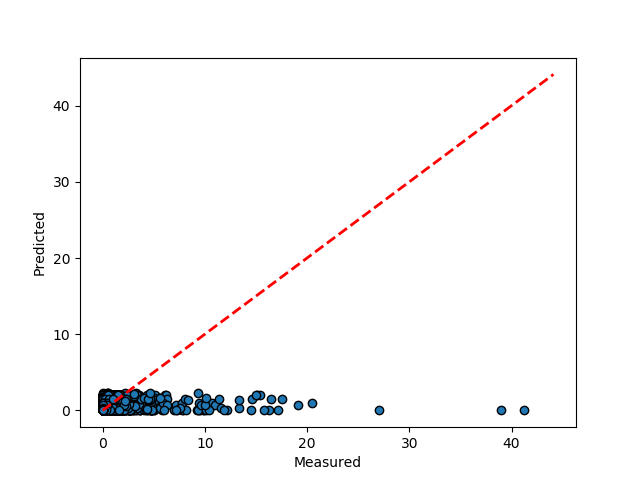
\includegraphics[width=0.8\textwidth]{media/opticeye_predictions.png}
	\caption{Shows the relationship between actual measurements and predictions made by kNN to predict precipitation amount. The closer a point is to the red dashed line, the more accurate prediction for that observation. }
	\label{fig:scatter_precamount}
\end{figure}

	Figure \ref{fig:scatter_precamount} shows a substantial difference between some measurements and predictions. Two measurements near 40 mm/30 min was predicted to be approximately 0 mm/30 min. The author suspected that some of the higher measurements of precipitation amount in the dataset was due to errors rather than being abnormal, but correct, measurements. The author consulted with Jonas Hallenberg at Trafikverket to see if some of the observations from the training dataset should be removed. Although he could not declare a definitive limit for a reasonable prediction amount, he recommended the author to set a limit at 20 mm/30 min \cite{MAIL:2}.

	The author decided to test an engineered version of the dataset in which all observations where precipitation amount is above 20 mm/30 min were removed, and run kNN again with the same settings as seen in table \ref{table:best_performances_precamount}. A total of 27 observations were removed, resulting in performance score $MSE_{newtest} = 0.31$ which is an improvement from $MSE_{test} = 0.54$. Although this experiment was conducted outside the frame of the experimental methodology of this project, it was decided to use its results as the new highest performance score: $MSE_{test} = 0.31$. Using the new results means that kNN was on average off by $\sqrt{0.31} \approx 0.56$ mm/30 min from the actual measurements in the test dataset.

\section{Predicting road surface temperature (DST111)}
	\subsection{Input features correlation ranking}

	\begin{table}[H]
		\centering
		\caption{Relevancy of each possible input features to the target feature: DST111 road surface temperature. }
		\begin{tabular}[3]{c | l | l }
    			Relevancy ranking & Input feature & Correlation score  \\
			 \hline
			1 & road surface condition & 11636.00 \\ \hline
			2 & road friction & 7411.80 \\ \hline
			3 & month & 4990.95 \\ \hline
			4 & precipitation type & 1897.37 \\ \hline
			5 & hour & 1784.49 \\ \hline
			6 & precipitation amount & 234,64 
 
			\label{table:feature_comparison_dst111}
		\end{tabular}
	\end{table}

	The correlation ranking from table \ref{table:feature_comparison_dst111} shows that road surface condition and road friction are the most relevant input features.

	\subsection{Spot-checking}
	\begin{table}[H]
		\centering
		\caption{Results from spot-checking experiment on the top features for predicting DST111 road surface temperature. The results are shown as a tuple: ($MSE_{test}$, $MSE_{diff}$) where $MSE_{test}$ represents performance and $MSE_{diff} = MSE_{test} - MSE_{train}$ shows the degree of overfitting, larger values of $MSE_{diff}$ indicate overfitting.}
		\resizebox{\textwidth}{!}{%
		\begin{tabular}[7]{l |c | c | c | c |c | c  }
    			Algorithm & top 6 features & top 5 features & top 4 features & top 3 features & top 2 features & top 1 features \\
			 \hline 
			OLS 			& (70.45, 0.20) & (70.50, 0.22) & (71.69, 0.21) & (71.70, 0.21) & (75.25, 0.06) & (75.64, 0.12) \\ \hline
			CART 		& (10.47, 1.54) & (10.27, 1.03) & (20.06, 0.50) & (20.56, 0.48) & (60.20, 0.01) & (60.93, -0.12) \\ \hline
			kNN 			& (11.83, 0.65) & (11.90, 0.82) & (22.60, 0.44) & (23.36, 0.34) & (62.68, -0.22) & (61.66, -0.13) \\ \hline
			MLP & (11.46, 0.27) & (13.14, 0.13) & (22.33, 0.34) & (22.44, 0.30) & (61.00, -0.15) & (62.49, -0.20) \\ \hline
			Lasso 		& (71.43, 0.19) & (71.43, 0.19) & (72.65, 0.20) & (72.65, 0.20) & (76.38, 0.04) & (76.38, 0.04) \\ \hline
			Random forest 	& (10.16, 1.11) & (10.16, 0.86) & (20.04, 0.46) & (20.56, 0.46) & (60.20, 0.00) & (60.93, -0.12) 
 
			\label{table:spotcheck_dst111}
		\end{tabular}
		}
	\end{table}
	
	\begin{table}[H]
		\centering
		\caption{Shows an accumalated performance score $P_{acc} = MSE_{test} + MSE_{diff}$. Top results for each algorithm are highlighted. In case of ties, the one using the fewest amount of input features is considered optimized. }
		\resizebox{\textwidth}{!}{%
		\begin{tabular}[7]{l |c | c | c | c |c | c  }
    			Algorithm &  $P_{acc}$ top 6 features& $P_{acc}$ top 5 features & $P_{acc}$ top 4 features & $P_{acc}$ top 3 features & $P_{acc}$ top 2 features & $P_{acc}$ top 1 features \\
			 \hline 
			OLS 			& \textbf{\underline{70.65}} & 70.72 & 71.90 & 71.91 & 75.31 & 75.52 \\ \hline
			CART 		& 12.01 & \textbf{\underline{11.30}} & 20.56 & 21.04 & 60.21 & 60.81 \\ \hline
			kNN 			& \textbf{\underline{12.48}} & 12.72 & 23.04 & 23.70 & 62.46 & 61.53 \\ \hline
			MLP & \textbf{\underline{11.73}} & 13.27 & 22.67 & 22.74 & 60.85 & 62.29 \\ \hline
			Lasso 		& \textbf{\underline{71.62}} & 71.63 & 72.85 & 72.85 & 76.42 & 76.42 \\ \hline
			Random forest 	& 11.27 & \textbf{\underline{11.02}} & 20.50 & 21.02 & 60.20 & 60.81 
 
			\label{table:spotcheck_dst111_acc}
		\end{tabular}
		}
	\end{table}

	The results from table \ref{table:spotcheck_dst111_acc} show that OLS, kNN, MLP and Lasso performs at best when all top six features are used, while CART and Random forest benefit most from using the top five features.

	\subsection{Optimizing hyperparameters}

	\begin{table}[H]
		\centering
		\caption{Shows the effect of optimizing the hyperparameters of kNN, MLP and Lasso using their top input features}
		\resizebox{\textwidth}{!}{%
		\begin{tabular}[6]{l |c | c | c | c | c }
    			Algorithm & Default hyperparameter setting & Optimized settings & Default performance $P_{acc}$ & optimized performance ($MSE_{test}$,$MSE_{diff}$) & optimized performance $P_{acc}$ \\
			\hline
			kNN 			& $k = 5$ & $k = 32$ & 12.48 & (10.69, 0.43) & 11.12 \\ \hline
 			MLP & n.o. hidden nodes: 100 & n.o. hidden nodes: 64 & 11.73 & (11.19, 0.29) & 11.48 \\ \hline
			Lasso		& $\lambda = 1$ & $\lambda = 0.001$ & 71.62 & (70.46, 0.21) & 70.67
			\label{table:optimization_dst111}
		\end{tabular}
		}
	\end{table}

	All three algorithms attain a slightly better $P_{acc}$ score in using their optimized hyperparameter settings. 

	\subsection{Results and analysis} \label{sec:results_dst111}

	\begin{table}[H]
		\centering
		\caption{Shows the overall optimized settings and performances for each of the algorithms in predicting DST111 road surface temperature. The best performing algorithm is highlighted. }
		\resizebox{\textwidth}{!}{%
		\begin{tabular}[5]{l |c | c | c  | c}
    			Algorithm & Optimized settings & Best choice of input features & Best performance ($MSE_{test}$, $MSE_{diff}$) & Best performance $P_{acc}$ \\
			\hline
			OLS 				& Scikit default & top 6 & (70.45, 0.20) & 70.65 \\ \hline
			CART 			& Scikit default & top 5 & (10.27, 1.03) & 11.30 \\ \hline
 			kNN 				& $k= 32$ & top 6 & (11.83, 0.65) & 12.48 \\ \hline
			MLP		& n.o. hidden nodes: 256 & top 6 & (11.46, 0.27) & 11.73 \\ \hline
			Lasso			& $\lambda = 0.001$ & top 6 & (71.43, 0.19) & 71.62 \\ \hline
			\textbf{\underline{Random forest}}		& \textbf{\underline{Scikit default}} & \textbf{\underline{top 5}} & \textbf{\underline{(10.16, 0.86)}} & \textbf{\underline{11.02}}
			\label{table:best_performances_dst111}
		\end{tabular}
		}
	\end{table}

		From table \ref{table:best_performances_dst111} it is revealed that Random forest has the lowest $P_{acc}$ score and is thus the best algorithm in predicting DST111 road surface temperature. The top performance score for random forest is $MSE_{test} =10.16$. This means that in predicting DST111 road surface temperature, the predictions made by Random forest was on average off by $\sqrt{10.16} \approx 3.19 \celsius$ from the actual temperature measurements in the test dataset. Figure \ref{fig:scatter_dst111} shows the relationship between predictions made by MLP on the test dataset and actual values. %lägg in plot som visar predictions

\begin{figure}[H] 
	\centering
	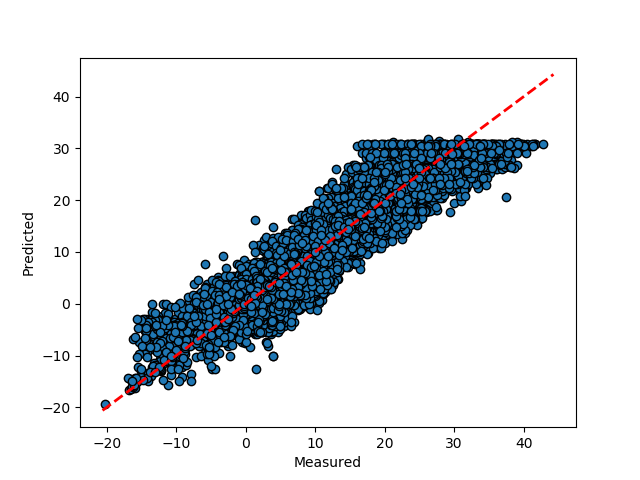
\includegraphics[width=0.8\textwidth]{media/dst111_predictions.png}
	\caption{Shows the relationship between actual measurements and predictions made by Random forest to predict DST111 road surface temperature. The closer a point is to the red dashed line, the more accurate prediction for that observation. }
	\label{fig:scatter_dst111}
\end{figure}

	Although DST111 and TIRS both measure road surface temperature, the optimal performances of the two have a substantial difference. Random forest was the best at predicting for the DST111 with a performance score of $MSE_{test} = 10.16$, and MLP was the best performer in predicting TIRS road surface temperature with a score of $MSE_{test} = 0.88$. One difference between the two tasks is that DST111 road surface temperature can be used as input feature to predict TIRS road surface temperature, but not the other way around (see thesis objective in \ref{sec:objective}). It was decided to test the importance of having road surface temperature as input feature to predict another road surface temperature. The results obtained were not used to solve the thesis subtasks, but rather to gain an understanding of why the two performance results differed by a large degree.

	Two holdout regression spot-checking experiments were carried out to see the importance of having either TIRS- or DST111 road surface temperature to predict the other. The first experiment is to predict TIRS road surface temperature but to not use its top relevant input feature: DST111 road surface temperature. The second experiment is to predict DST111 road surface temperature allowing TIRS road surface temperature to be used as input feature. In this project, top performance for predicting TIRS road surface temperature was $MSE_{test} = 0.88$, this was when DST111 was allowed as input feature. When not using DST111 as input feature, the best performance among algorithms to predict TIRS road surface temperature was Random forest with a reduced performance score of $MSE_{test}=15.36$. In the case of predicting DST111 road surface temperature, it was not allowed to use TIRS road surface temperature as input feature in this project, resulting in a performance score of $MSE_{test}=10.16$. In allowing TIRS to be used as input feature in this experiment, the best performing algorithm to predict DST111 road surface temperature was MLP with a performance score of $MSE_{test}=0.77$. 

